\documentclass[10pt,a4paper]{article}
% Shared journal-style layout for main.tex and supplement.tex (compiled with tectonic by scripts/build_paper.py).
% Each document sets its own \documentclass and \geometry before and after % Shared journal-style layout for main.tex and supplement.tex (compiled with tectonic by scripts/build_paper.py).
% Each document sets its own \documentclass and \geometry before and after % Shared journal-style layout for main.tex and supplement.tex (compiled with tectonic by scripts/build_paper.py).
% Each document sets its own \documentclass and \geometry before and after \input{preamble}.
\usepackage{geometry}
\usepackage{fontspec}
\setmainfont{Charter}
\setsansfont{Helvetica Neue}[BoldFont={Helvetica Neue Bold}, ItalicFont={Helvetica Neue Italic},
  BoldItalicFont={Helvetica Neue Bold Italic}]
\usepackage{microtype}
\usepackage[table]{xcolor}
\usepackage{booktabs,tabularx,graphicx,array,makecell,longtable}
\usepackage{float}
\usepackage{enumitem}
\usepackage{etoolbox}
\usepackage{tikz}
\usetikzlibrary{positioning,calc}
\usepackage{titlesec}
\usepackage{fancyhdr}
\usepackage[numbers,sort&compress]{natbib}
\usepackage{caption}
\usepackage{hyperref}
\usepackage{xurl}

\definecolor{accent}{HTML}{1B4F72}
\definecolor{accentlight}{HTML}{EAF1F7}
\definecolor{tablehead}{HTML}{DCE7F1}
\hypersetup{colorlinks=true, linkcolor=accent, citecolor=accent, urlcolor=accent}
\urlstyle{same}

% Text
\setlength{\parindent}{1em}
\setlength{\parskip}{0pt}
\setlist{nosep,leftmargin=1.2em}
\titleformat{\section}{\sffamily\bfseries\large\color{accent}}{}{0pt}{}
\titleformat{\subsection}{\sffamily\bfseries\normalsize}{}{0pt}{}
\titlespacing*{\section}{0pt}{1.1em}{0.35em}
\titlespacing*{\subsection}{0pt}{0.7em}{0.15em}
\newcommand{\abshead}[1]{{\sffamily\bfseries\footnotesize\color{accent}\MakeUppercase{#1}}\enspace}

% Floats: sans-serif tables with a shaded header row, captions above tables
\captionsetup{font={footnotesize,sf}, labelfont={bf}, labelsep=period, justification=raggedright,
  singlelinecheck=false}
\captionsetup[table]{position=top, skip=4pt}
\AtBeginEnvironment{table}{\sffamily}
\AtBeginEnvironment{table*}{\sffamily}
\AtBeginEnvironment{longtable}{\sffamily}
\setlength{\aboverulesep}{0pt}
\setlength{\belowrulesep}{0pt}
\setlength{\extrarowheight}{1.6pt}
\arrayrulecolor{accent}
\setlength{\textfloatsep}{12pt plus 2pt minus 2pt}
\setlength{\dbltextfloatsep}{12pt plus 2pt minus 2pt}

% References
\renewcommand{\refname}{References}
\renewcommand{\bibfont}{\footnotesize}
\setlength{\bibsep}{1.2pt}

% Running heads and feet
\newcommand{\shorttitle}{Predicting prostate cancer treatment delays of more than 90 days}
\newcommand{\docversion}{Version 1, 14 September 2026}
\newcommand{\doclabel}{Preprint}
\newcommand{\footline}{\sffamily\scriptsize\textcolor{black!55}{\docversion}}
\fancypagestyle{journal}{%
  \fancyhf{}%
  \fancyhead[L]{\sffamily\scriptsize\textcolor{accent}{\bfseries\MakeUppercase{\doclabel}}\quad
    \textcolor{black!65}{\shorttitle}}%
  \fancyhead[R]{\sffamily\scriptsize\textcolor{black!65}{Hinge}}%
  \fancyfoot[L]{\footline}%
  \fancyfoot[R]{\sffamily\scriptsize\bfseries\thepage}%
  \renewcommand{\headrulewidth}{0.5pt}%
  \renewcommand{\headrule}{{\color{accent}\hrule height 0.5pt width \headwidth \vskip -0.5pt}}}
\fancypagestyle{firstpage}{%
  \fancyhf{}%
  \fancyfoot[L]{\footline}%
  \fancyfoot[R]{\sffamily\scriptsize\bfseries\thepage}%
  \renewcommand{\headrulewidth}{0pt}%
  \renewcommand{\headrule}{}}
\pagestyle{journal}

% Coloured band across the top of the first page
\newcommand{\topband}[2]{\noindent\colorbox{accent}{\parbox{\dimexpr\textwidth-2\fboxsep}{%
  \sffamily\footnotesize\bfseries\color{white}\strut #1\hfill #2}}}
.
\usepackage{geometry}
\usepackage{fontspec}
\setmainfont{Charter}
\setsansfont{Helvetica Neue}[BoldFont={Helvetica Neue Bold}, ItalicFont={Helvetica Neue Italic},
  BoldItalicFont={Helvetica Neue Bold Italic}]
\usepackage{microtype}
\usepackage[table]{xcolor}
\usepackage{booktabs,tabularx,graphicx,array,makecell,longtable}
\usepackage{float}
\usepackage{enumitem}
\usepackage{etoolbox}
\usepackage{tikz}
\usetikzlibrary{positioning,calc}
\usepackage{titlesec}
\usepackage{fancyhdr}
\usepackage[numbers,sort&compress]{natbib}
\usepackage{caption}
\usepackage{hyperref}
\usepackage{xurl}

\definecolor{accent}{HTML}{1B4F72}
\definecolor{accentlight}{HTML}{EAF1F7}
\definecolor{tablehead}{HTML}{DCE7F1}
\hypersetup{colorlinks=true, linkcolor=accent, citecolor=accent, urlcolor=accent}
\urlstyle{same}

% Text
\setlength{\parindent}{1em}
\setlength{\parskip}{0pt}
\setlist{nosep,leftmargin=1.2em}
\titleformat{\section}{\sffamily\bfseries\large\color{accent}}{}{0pt}{}
\titleformat{\subsection}{\sffamily\bfseries\normalsize}{}{0pt}{}
\titlespacing*{\section}{0pt}{1.1em}{0.35em}
\titlespacing*{\subsection}{0pt}{0.7em}{0.15em}
\newcommand{\abshead}[1]{{\sffamily\bfseries\footnotesize\color{accent}\MakeUppercase{#1}}\enspace}

% Floats: sans-serif tables with a shaded header row, captions above tables
\captionsetup{font={footnotesize,sf}, labelfont={bf}, labelsep=period, justification=raggedright,
  singlelinecheck=false}
\captionsetup[table]{position=top, skip=4pt}
\AtBeginEnvironment{table}{\sffamily}
\AtBeginEnvironment{table*}{\sffamily}
\AtBeginEnvironment{longtable}{\sffamily}
\setlength{\aboverulesep}{0pt}
\setlength{\belowrulesep}{0pt}
\setlength{\extrarowheight}{1.6pt}
\arrayrulecolor{accent}
\setlength{\textfloatsep}{12pt plus 2pt minus 2pt}
\setlength{\dbltextfloatsep}{12pt plus 2pt minus 2pt}

% References
\renewcommand{\refname}{References}
\renewcommand{\bibfont}{\footnotesize}
\setlength{\bibsep}{1.2pt}

% Running heads and feet
\newcommand{\shorttitle}{Predicting prostate cancer treatment delays of more than 90 days}
\newcommand{\docversion}{Version 1, 14 September 2026}
\newcommand{\doclabel}{Preprint}
\newcommand{\footline}{\sffamily\scriptsize\textcolor{black!55}{\docversion}}
\fancypagestyle{journal}{%
  \fancyhf{}%
  \fancyhead[L]{\sffamily\scriptsize\textcolor{accent}{\bfseries\MakeUppercase{\doclabel}}\quad
    \textcolor{black!65}{\shorttitle}}%
  \fancyhead[R]{\sffamily\scriptsize\textcolor{black!65}{Hinge}}%
  \fancyfoot[L]{\footline}%
  \fancyfoot[R]{\sffamily\scriptsize\bfseries\thepage}%
  \renewcommand{\headrulewidth}{0.5pt}%
  \renewcommand{\headrule}{{\color{accent}\hrule height 0.5pt width \headwidth \vskip -0.5pt}}}
\fancypagestyle{firstpage}{%
  \fancyhf{}%
  \fancyfoot[L]{\footline}%
  \fancyfoot[R]{\sffamily\scriptsize\bfseries\thepage}%
  \renewcommand{\headrulewidth}{0pt}%
  \renewcommand{\headrule}{}}
\pagestyle{journal}

% Coloured band across the top of the first page
\newcommand{\topband}[2]{\noindent\colorbox{accent}{\parbox{\dimexpr\textwidth-2\fboxsep}{%
  \sffamily\footnotesize\bfseries\color{white}\strut #1\hfill #2}}}
.
\usepackage{geometry}
\usepackage{fontspec}
\setmainfont{Charter}
\setsansfont{Helvetica Neue}[BoldFont={Helvetica Neue Bold}, ItalicFont={Helvetica Neue Italic},
  BoldItalicFont={Helvetica Neue Bold Italic}]
\usepackage{microtype}
\usepackage[table]{xcolor}
\usepackage{booktabs,tabularx,graphicx,array,makecell,longtable}
\usepackage{float}
\usepackage{enumitem}
\usepackage{etoolbox}
\usepackage{tikz}
\usetikzlibrary{positioning,calc}
\usepackage{titlesec}
\usepackage{fancyhdr}
\usepackage[numbers,sort&compress]{natbib}
\usepackage{caption}
\usepackage{hyperref}
\usepackage{xurl}

\definecolor{accent}{HTML}{1B4F72}
\definecolor{accentlight}{HTML}{EAF1F7}
\definecolor{tablehead}{HTML}{DCE7F1}
\hypersetup{colorlinks=true, linkcolor=accent, citecolor=accent, urlcolor=accent}
\urlstyle{same}

% Text
\setlength{\parindent}{1em}
\setlength{\parskip}{0pt}
\setlist{nosep,leftmargin=1.2em}
\titleformat{\section}{\sffamily\bfseries\large\color{accent}}{}{0pt}{}
\titleformat{\subsection}{\sffamily\bfseries\normalsize}{}{0pt}{}
\titlespacing*{\section}{0pt}{1.1em}{0.35em}
\titlespacing*{\subsection}{0pt}{0.7em}{0.15em}
\newcommand{\abshead}[1]{{\sffamily\bfseries\footnotesize\color{accent}\MakeUppercase{#1}}\enspace}

% Floats: sans-serif tables with a shaded header row, captions above tables
\captionsetup{font={footnotesize,sf}, labelfont={bf}, labelsep=period, justification=raggedright,
  singlelinecheck=false}
\captionsetup[table]{position=top, skip=4pt}
\AtBeginEnvironment{table}{\sffamily}
\AtBeginEnvironment{table*}{\sffamily}
\AtBeginEnvironment{longtable}{\sffamily}
\setlength{\aboverulesep}{0pt}
\setlength{\belowrulesep}{0pt}
\setlength{\extrarowheight}{1.6pt}
\arrayrulecolor{accent}
\setlength{\textfloatsep}{12pt plus 2pt minus 2pt}
\setlength{\dbltextfloatsep}{12pt plus 2pt minus 2pt}

% References
\renewcommand{\refname}{References}
\renewcommand{\bibfont}{\footnotesize}
\setlength{\bibsep}{1.2pt}

% Running heads and feet
\newcommand{\shorttitle}{Predicting prostate cancer treatment delays of more than 90 days}
\newcommand{\docversion}{Version 1, 14 September 2026}
\newcommand{\doclabel}{Preprint}
\newcommand{\footline}{\sffamily\scriptsize\textcolor{black!55}{\docversion}}
\fancypagestyle{journal}{%
  \fancyhf{}%
  \fancyhead[L]{\sffamily\scriptsize\textcolor{accent}{\bfseries\MakeUppercase{\doclabel}}\quad
    \textcolor{black!65}{\shorttitle}}%
  \fancyhead[R]{\sffamily\scriptsize\textcolor{black!65}{Hinge}}%
  \fancyfoot[L]{\footline}%
  \fancyfoot[R]{\sffamily\scriptsize\bfseries\thepage}%
  \renewcommand{\headrulewidth}{0.5pt}%
  \renewcommand{\headrule}{{\color{accent}\hrule height 0.5pt width \headwidth \vskip -0.5pt}}}
\fancypagestyle{firstpage}{%
  \fancyhf{}%
  \fancyfoot[L]{\footline}%
  \fancyfoot[R]{\sffamily\scriptsize\bfseries\thepage}%
  \renewcommand{\headrulewidth}{0pt}%
  \renewcommand{\headrule}{}}
\pagestyle{journal}

% Coloured band across the top of the first page
\newcommand{\topband}[2]{\noindent\colorbox{accent}{\parbox{\dimexpr\textwidth-2\fboxsep}{%
  \sffamily\footnotesize\bfseries\color{white}\strut #1\hfill #2}}}

\geometry{top=21mm, bottom=22mm, left=20mm, right=20mm, headsep=5mm, footskip=9mm}
\renewcommand{\doclabel}{Supplementary material}
\setlength{\parindent}{0pt}
\setlength{\parskip}{0.45em}
\renewcommand{\thetable}{S\arabic{table}}
\renewcommand{\thefigure}{S\arabic{figure}}

\begin{document}

\thispagestyle{firstpage}
\topband{SUPPLEMENTARY MATERIAL \textbar{} HEALTH SERVICES RESEARCH AND MACHINE LEARNING}{PREPRINT VERSION}

\vspace{12pt}
{\raggedright\sffamily\bfseries\fontsize{16}{20}\selectfont Predicting treatment delays of more than 90 days in prostate cancer: added value of county rurality, county income and marital status over clinical characteristics\par}
\vspace{4pt}
{\raggedright\sffamily\large\color{black!70} A machine learning cohort study of 330,827 men treated with surgery or radiotherapy in US SEER registries, 2010 to 2022\par}
\vspace{8pt}
{\raggedright\sffamily\small\textbf{Tanmay Hinge}\enspace\textcolor{black!70}{Code, protocol and full analysis reports: \url{https://github.com/tanmayhinge/seer-prostate}}\par}
\vspace{8pt}
{\color{accent}\hrule height 0.8pt}
\vspace{4pt}

\section{How to read this supplement}
\begin{itemize}
\item \textbf{Source of tables.} Every table is generated by script from the analysis reports in the public repository, so the values match the analysis outputs. The reports, in the \texttt{reports} folder, contain further tables not reproduced here, including results for every model step, leave-one-variable-out refits, bounds by income and marital status, and the protocol amendment log.
\item \textbf{Skill and intervals.} Skill added is in percentage points of out-of-fold log-loss skill. Intervals are 95\% cluster bootstrap intervals over rurality by county income cells (500 resamples of out-of-fold predictions, no refitting) unless stated, so they exclude model-fitting variability.
\item \textbf{Disclosure control.} As the SEER Research Data Use Agreement requires, statistics resting on 1 to 4 men are shown as $<$5, and numbers of men in cross-tabulations are rounded to the nearest 10.
\item \textbf{Later robustness analyses.} Tables S3 and S4 and the indices by period in Table S7 come from analyses added by protocol amendment 1.9 and specified before they were run. The two-model agreement rule for standardised contrasts was adopted post hoc (amendment 1.7).
\end{itemize}

\section{Box S1. Survival comparisons and immortal time bias (not estimated)}
Comparing survival between treated and untreated men is exposed to immortal time bias, because treated men must survive until treatment starts. A simulation study of observational research found that time-fixed and exclusion methods overestimated a treatment's benefit, that a 1-year landmark method reduced the bias but did not remove it, and recommended the time-dependent method~\cite{zheng2023}. A suitable design would treat treatment as a time-dependent exposure, with competing risks of prostate cancer death and death from other causes, and use a 12-month landmark analysis only as a sensitivity analysis. This design is described, not estimated, in this study.

\section{Box S2. Candidate Australian analogues of the SEER variables (no Australian data analysed)}
Published analyses of the Prostate Cancer Outcomes Registry in Tasmania used the measures below~\cite{foley2022,foley2025}. They are candidate analogues, not equivalents: the geographic units, the construction of the measures and the health systems differ, and availability for any new study must be confirmed against the registry's data dictionary.
\begin{itemize}
\item \textbf{Rurality.} The county Rural-Urban Continuum Code has a candidate analogue in Australian Statistical Geography Standard remoteness areas, assigned by residential postcode.
\item \textbf{Area income.} County median household income has a candidate analogue in the SEIFA Index of Relative Socio-Economic Advantage and Disadvantage, assigned by postcode.
\item \textbf{Insurance and sector.} SEER has no insurance variable. The closest Australian contrast studied is a public or private treating facility.
\end{itemize}
Data gaps reported in those analyses were no comorbidity data~\cite{foley2022}, patient-reported outcomes collected consistently only from 2018~\cite{foley2025}, and no way to tell whether external beam radiotherapy was given in a public or private facility~\cite{foley2025}. Referral, biopsy and multidisciplinary meeting dates are not assumed to be available.

\section{Supplementary tables}

\begin{table}[H]
\centering
\footnotesize
\setlength{\tabcolsep}{3pt}
\caption{Crude waiting beyond 90 days by risk group and county rurality}
\label{tab:s1}
\begin{tabular}{@{}llrrrr@{}}
\toprule
\makecell[l]{Risk group} & \makecell[l]{County rurality} & \makecell[r]{Men} & \makecell[r]{Waited more\\than 90 days (\%)} & \makecell[r]{Median\\days} & \makecell[r]{90th percentile\\days} \\
\midrule
Low & Metro, 1 million or more & 34,260 & 50.7 & 91 & 217 \\
 & Metro, 250,000 to 1 million & 11,930 & 47.0 & 86 & 211 \\
 & Metro, under 250,000 & 4,780 & 42.3 & 82 & 198.2 \\
 & Nonmetro, adjacent to metro & 3,990 & 39.0 & 77 & 187 \\
 & Nonmetro, not adjacent to metro & 2,510 & 39.0 & 76 & 177 \\
 & Unknown & 20 & 34.8 & 81 & 122.8 \\
Intermediate & Metro, 1 million or more & 75,190 & 45.5 & 84 & 182 \\
 & Metro, 250,000 to 1 million & 28,140 & 41.1 & 79 & 172 \\
 & Metro, under 250,000 & 10,070 & 36.7 & 75 & 165 \\
 & Nonmetro, adjacent to metro & 8,830 & 36.1 & 74 & 161 \\
 & Nonmetro, not adjacent to metro & 5,360 & 36.1 & 71 & 160 \\
 & Unknown & 40 & 42.5 & 71 & 200.5 \\
High & Metro, 1 million or more & 75,760 & 35.7 & 73 & 157 \\
 & Metro, 250,000 to 1 million & 29,320 & 30.0 & 67 & 142 \\
 & Metro, under 250,000 & 10,130 & 27.9 & 65 & 140 \\
 & Nonmetro, adjacent to metro & 9,590 & 27.7 & 63 & 134.5 \\
 & Nonmetro, not adjacent to metro & 6,010 & 26.0 & 62 & 133 \\
 & Unknown & 90 & 28.4 & 61.5 & 141.5 \\
Unknown & Metro, 1 million or more & 9,460 & 44.2 & 82 & 224 \\
 & Metro, 250,000 to 1 million & 2,770 & 42.2 & 80 & 203 \\
 & Metro, under 250,000 & 1,120 & 35.0 & 70 & 179 \\
 & Nonmetro, adjacent to metro & 950 & 36.5 & 72 & 174.2 \\
 & Nonmetro, not adjacent to metro & 510 & 29.6 & 63.5 & 162 \\
 & Unknown & 10 & $<$5 & 77 & 212.7 \\
\bottomrule
\end{tabular}
\par\smallskip
\begin{minipage}{\linewidth}\scriptsize Crude values; nothing is adjusted. Numbers of men are rounded to the nearest 10. Medians and 90th percentiles count top-coded intervals as 731 days. $<$5: statistic suppressed because 1 to 4 men in the row did, or did not, wait more than 90 days.\end{minipage}
\end{table}

\begin{table}[H]
\centering
\footnotesize
\setlength{\tabcolsep}{3pt}
\caption{Performance at step 2 by risk group and model}
\label{tab:s2}
\begin{tabular}{@{}llrrrrr@{}}
\toprule
\makecell[l]{Stratum} & \makecell[l]{Model} & \makecell[r]{Log-loss\\skill (\%)} & \makecell[r]{Brier\\skill (\%)} & \makecell[r]{AUC} & \makecell[r]{Calibration\\intercept} & \makecell[r]{Calibration\\slope} \\
\midrule
All men & Logistic & 3.63 & 4.66 & 0.638 & $-$0.000 & 1.000 \\
 & LightGBM & 4.17 & 5.34 & 0.648 & $-$0.000 & 1.030 \\
Low risk & Logistic & 0.76 & 1.03 & 0.592 & 0.000 & 0.988 \\
 & LightGBM & 0.99 & 1.35 & 0.604 & $-$0.000 & 0.937 \\
Intermediate risk & Logistic & 1.06 & 1.40 & 0.605 & $-$0.000 & 1.001 \\
 & LightGBM & 1.48 & 1.96 & 0.615 & $-$0.000 & 1.008 \\
High risk & Logistic & 4.39 & 5.42 & 0.654 & 0.000 & 1.001 \\
 & LightGBM & 4.90 & 6.04 & 0.663 & $-$0.000 & 1.023 \\
Unknown risk & Logistic & 1.07 & 1.43 & 0.610 & 0.000 & 0.982 \\
 & LightGBM & 1.96 & 2.64 & 0.629 & $-$0.000 & 0.882 \\
\bottomrule
\end{tabular}
\par\smallskip
\begin{minipage}{\linewidth}\scriptsize Out-of-fold predictions at step 2 (clinical need plus area and marital characteristics). Skill is against the step 0 model. Calibration intercept: 0 is ideal; slope: 1 is ideal, below 1 means predictions are too extreme. Values for every step are in \texttt{reports/phase4\_models.md}.\end{minipage}
\end{table}

\begin{table}[H]
\centering\sffamily
\footnotesize
\setlength{\tabcolsep}{2pt}
\caption{Robustness of the area and marital increment to tuning, fold assignment and clustering}
\label{tab:s3}
\begin{tabular}{@{}llrrrr@{}}
\toprule
\rowcolor{tablehead}\makecell[l]{Stratum} & \makecell[l]{Model} & \makecell[r]{Primary analysis\\(tuned at step 3)} & \makecell[r]{Tuned at\\each step} & \makecell[r]{Mean (range) over\\10 fold seeds} & \makecell[r]{Clustered by county\\income band only} \\
\midrule
All men & Logistic & 0.62 (0.39 to 0.87) & 0.62 (0.39 to 0.87) & 0.62 (0.61 to 0.62) & 0.62 (0.38 to 0.90) \\
 & LightGBM & 0.99 (0.73 to 1.30) & 0.99 (0.73 to 1.30) & 0.99 (0.98 to 0.99) & 0.99 (0.72 to 1.35) \\
Low risk & Logistic & 0.62 (0.32 to 0.94) & 0.62 (0.32 to 0.94) & 0.62 (0.59 to 0.63) & 0.62 (0.28 to 1.07) \\
 & LightGBM & 0.96 (0.67 to 1.28) & 0.96 (0.67 to 1.28) & 0.98 (0.95 to 1.01) & 0.96 (0.64 to 1.36) \\
Intermediate risk & Logistic & 0.56 (0.35 to 0.83) & 0.56 (0.34 to 0.83) & 0.56 (0.54 to 0.56) & 0.56 (0.33 to 0.89) \\
 & LightGBM & 0.93 (0.65 to 1.27) & 0.93 (0.65 to 1.27) & 0.93 (0.91 to 0.97) & 0.93 (0.63 to 1.31) \\
High risk & Logistic & 0.86 (0.60 to 1.15) & 0.86 (0.60 to 1.15) & 0.85 (0.85 to 0.86) & 0.86 (0.58 to 1.15) \\
 & LightGBM & 1.18 (0.90 to 1.56) & 1.18 (0.90 to 1.54) & 1.18 (1.16 to 1.20) & 1.18 (0.87 to 1.55) \\
Unknown risk & Logistic & 0.42 (0.08 to 0.80) & 0.40 (0.07 to 0.80) & 0.41 (0.32 to 0.48) & 0.40 (0.07 to 0.78) \\
 & LightGBM & 1.37 (0.80 to 2.19) & 1.37 (0.80 to 2.19) & 1.29 (1.22 to 1.43) & 1.37 (0.78 to 2.09) \\
\bottomrule
\end{tabular}
\par\smallskip
\begin{minipage}{\linewidth}\scriptsize Percentage points of out-of-fold log-loss skill added by area and marital characteristics (step 1 to 2), with 95\% cluster bootstrap intervals (first fold seed, 500 resamples, no refitting). Tuning was not repeated per seed. Specified after an internal review (protocol amendment 1.9).\end{minipage}
\end{table}

\begin{table}[H]
\centering\sffamily
\footnotesize
\setlength{\tabcolsep}{3pt}
\caption{Stage-free clinical block and year of diagnosis as categories}
\label{tab:s4}
\begin{tabular}{@{}lllrr@{}}
\toprule
\rowcolor{tablehead}\makecell[l]{Analysis} & \makecell[l]{Stratum} & \makecell[l]{Model} & \makecell[r]{Clinical need added\\(95\% interval)} & \makecell[r]{Area and marital added\\(95\% interval)} \\
\midrule
Stage-free clinical block & All men & Logistic & 2.97 (2.64 to 3.34) & 0.62 (0.39 to 0.87) \\
 &  & LightGBM & 3.13 (2.80 to 3.48) & 1.02 (0.75 to 1.33) \\
 & Low risk & Logistic & 0.14 (0.08 to 0.20) & 0.62 (0.32 to 0.94) \\
 &  & LightGBM & 0.02 ($-$0.09 to 0.13) & 0.96 (0.67 to 1.28) \\
 & Intermediate risk & Logistic & 0.49 (0.41 to 0.57) & 0.56 (0.34 to 0.83) \\
 &  & LightGBM & 0.55 (0.44 to 0.65) & 0.93 (0.65 to 1.27) \\
 & High risk & Logistic & 3.42 (3.07 to 3.76) & 0.85 (0.59 to 1.14) \\
 &  & LightGBM & 3.64 (3.27 to 3.99) & 1.19 (0.91 to 1.57) \\
 & Unknown risk & Logistic & 0.66 (0.41 to 0.92) & 0.40 (0.06 to 0.80) \\
 &  & LightGBM & 0.59 (0.27 to 0.95) & 1.37 (0.80 to 2.19) \\
Year as categories & All men & Logistic & 2.98 (2.66 to 3.34) & 0.62 (0.39 to 0.86) \\
 & Low risk & Logistic & 0.15 (0.09 to 0.21) & 0.60 (0.31 to 0.92) \\
 & Intermediate risk & Logistic & 0.50 (0.42 to 0.58) & 0.56 (0.34 to 0.83) \\
 & High risk & Logistic & 3.48 (3.12 to 3.82) & 0.87 (0.61 to 1.16) \\
 & Unknown risk & Logistic & 0.65 (0.41 to 0.90) & 0.47 (0.11 to 0.89) \\
\bottomrule
\end{tabular}
\par\smallskip
\begin{minipage}{\linewidth}\scriptsize Stage-free: summary stage removed from the clinical block, risk strata unchanged. Year as categories: logistic regression only, one indicator per year replacing linear year and the 2020 indicator. Both use per-step tuning and the first fold seed. Primary estimates are in Table 2 of the main text. Added by protocol amendment 1.9 and specified before being run.\end{minipage}
\end{table}

\begin{table}[H]
\centering
\scriptsize
\setlength{\tabcolsep}{3pt}
\caption{Sensitivity analyses}
\label{tab:s5}
\begin{tabular}{@{}>{\raggedright\arraybackslash}p{3.2cm}rrrrrrr@{}}
\toprule
\makecell[l]{Scenario} & \makecell[r]{Threshold\\(days)} & \makecell[r]{Men} & \makecell[r]{Delayed\\(\%)} & \makecell[r]{Added, logistic\\(95\% interval)} & \makecell[r]{Added, LightGBM\\(95\% interval)} & \makecell[r]{Area\\contrast} & \makecell[r]{Never married\\contrast} \\
\midrule
Primary analysis & 90 & 330,830 & 39.7 & 0.62 (0.39 to 0.87) & 0.99 (0.73 to 1.30) & $-$9.2 / $-$8.8 & 6.7 / 5.9 \\
Threshold of 60 days & 60 & 330,830 & 66.6 & 0.54 (0.31 to 0.79) & 0.94 (0.73 to 1.18) & $-$10.6 / $-$10.3 & 3.7 / 3.2 \\
Threshold of 120 days & 120 & 330,830 & 23.0 & 0.68 (0.45 to 0.93) & 1.06 (0.79 to 1.38) & $-$6.9 / $-$7.1 & 6.0 / 5.0 \\
Threshold of 180 days & 180 & 330,830 & 9.1 & 0.66 (0.41 to 0.92) & 1.00 (0.69 to 1.35) & $-$3.0 / $-$3.2\textsuperscript{a} & 3.4 / 3.1 \\
Risk groups from Gleason score and PSA only & 90 & 330,830 & 39.7 & 0.62 (0.39 to 0.87) & 0.99 (0.73 to 1.30) & $-$9.2 / $-$8.8 & 6.7 / 5.9 \\
Radical prostatectomy without radiotherapy only & 90 & 159,580 & 41.1 & 0.66 (0.48 to 0.88) & 1.00 (0.79 to 1.26) & $-$8.9 / $-$7.8 & 7.1 / 6.9 \\
Excluding men diagnosed in 2020 & 90 & 306,960 & 39.6 & 0.64 (0.40 to 0.91) & 1.03 (0.75 to 1.35) & $-$9.4 / $-$8.9 & 6.8 / 5.9 \\
Including men diagnosed in 2023 & 90 & 358,540 & 40.8 & 0.56 (0.35 to 0.80) & 0.94 (0.69 to 1.22) & $-$8.6 / $-$8.3 & 6.4 / 5.8 \\
Including intervals of 0 days & 90 & 338,580 & 38.8 & 0.61 (0.38 to 0.86) & 0.97 (0.70 to 1.27) & $-$9.2 / $-$9.2 & 6.5 / 5.8 \\
One primary cancer only (strict first primary) & 90 & 296,120 & 40.1 & 0.61 (0.38 to 0.85) & 0.98 (0.73 to 1.27) & $-$9.1 / $-$9.3 & 6.6 / 5.6 \\
Excluding prostatectomy not otherwise specified & 90 & 330,180 & 39.7 & 0.62 (0.39 to 0.87) & 0.98 (0.72 to 1.28) & $-$9.2 / $-$9.1 & 6.7 / 5.9 \\
\bottomrule
\end{tabular}
\par\smallskip
\begin{minipage}{\linewidth}\scriptsize All men. Each scenario changes one setting from the primary analysis. Added: percentage points of log-loss skill added by area and marital characteristics. Contrasts are standardised differences in percentage points (logistic / LightGBM): nonmetro counties not adjacent to a metro area minus metro areas of 1 million or more, each at its typical county income; and never married minus married. \textsuperscript{a}Two-model rule (both 3 points or more, same direction) not met. Threshold scenarios use a different outcome, so their values are not directly comparable. Numbers of men are rounded to the nearest 10.\end{minipage}
\end{table}

\begin{table}[H]
\centering\sffamily
\footnotesize
\setlength{\tabcolsep}{3pt}
\caption{Standardised contrasts in waiting more than 90 days, by risk group}
\label{tab:s6}
\begin{tabular}{@{}llrrl@{}}
\toprule
\rowcolor{tablehead}\makecell[l]{Stratum} & \makecell[l]{Contrast} & \makecell[r]{Logistic} & \makecell[r]{LightGBM} & \makecell[l]{Two-model\\rule met} \\
\midrule
All men & Observed minus reference profile & $-$1.1 & $-$1.6 & no, both under 3 \\
 & Nonmetro not adjacent minus metro 1 million or more & $-$9.2 & $-$8.8 & yes \\
 & Never married minus married & 6.7 & 5.9 & yes \\
Low risk & Observed minus reference profile & $-$3.4 & $-$4.7 & yes \\
 & Nonmetro not adjacent minus metro 1 million or more & $-$11.3 & $-$13.5 & yes \\
 & Never married minus married & 3.6 & 2.4 & no, one model only \\
Intermediate risk & Observed minus reference profile & $-$1.4 & $-$1.6 & no, both under 3 \\
 & Nonmetro not adjacent minus metro 1 million or more & $-$8.7 & $-$9.5 & yes \\
 & Never married minus married & 6.4 & 5.5 & yes \\
High risk & Observed minus reference profile & 0.1 & $-$0.1 & no, both under 3 \\
 & Nonmetro not adjacent minus metro 1 million or more & $-$8.4 & $-$7.2 & yes \\
 & Never married minus married & 8.3 & 7.6 & yes \\
Unknown risk & Observed minus reference profile & $-$0.1 & 0.0 & no, both under 3 \\
 & Nonmetro not adjacent minus metro 1 million or more & $-$12.1 & $-$14.2 & yes \\
 & Never married minus married & 6.0 & 6.2 & yes \\
\bottomrule
\end{tabular}
\par\smallskip
\begin{minipage}{\linewidth}\scriptsize Standardised percentage points waiting more than 90 days (g-computation with the step 2 model; each man keeps his own clinical features and year). Reference profile: married, metro area of 1 million or more, county income rank at the 83.33\% quantile. Area profiles set rurality and county income together at the median income band of men living in that type of area. Rule (post hoc, amendment 1.7): both models 3 points or more in the same direction. No intervals are reported.\end{minipage}
\end{table}

\begin{table}[H]
\centering\sffamily
\footnotesize
\setlength{\tabcolsep}{3pt}
\caption{Income concentration of delay, overall and by period of diagnosis}
\label{tab:s7}
\begin{tabular}{@{}lrrrr@{}}
\toprule
\rowcolor{tablehead}\makecell[l]{Stratum} & \makecell[r]{2010 to 2022} & \makecell[r]{2010 to 2014} & \makecell[r]{2015 to 2019} & \makecell[r]{2020 to 2022} \\
\midrule
All men & 0.062 (0.039 to 0.083) & 0.059 (0.025 to 0.092) & 0.037 (0.011 to 0.065) & 0.027 (0.003 to 0.061) \\
Low risk & 0.103 (0.068 to 0.134) & 0.092 (0.053 to 0.136) & 0.084 (0.052 to 0.121) & 0.052 (0.017 to 0.092) \\
Intermediate risk & 0.075 (0.051 to 0.096) & 0.058 (0.023 to 0.099) & 0.048 (0.019 to 0.080) & 0.039 (0.015 to 0.067) \\
High risk & 0.041 (0.017 to 0.065) & 0.028 ($-$0.011 to 0.062) & 0.020 ($-$0.004 to 0.049) & 0.015 ($-$0.013 to 0.056) \\
Unknown risk & 0.077 (0.037 to 0.128) & 0.060 (0.001 to 0.130) & 0.023 ($-$0.041 to 0.100) & 0.049 ($-$0.005 to 0.101) \\
\bottomrule
\end{tabular}
\par\smallskip
\begin{minipage}{\linewidth}\scriptsize Erreygers-corrected concentration index (95\% cluster bootstrap interval) of waiting more than 90 days, ranking men by county median household income, poorest first. Positive values mean delay is concentrated in higher-income counties. Crude: not standardised for clinical features, and it does not separate income from rurality. Indices by period were specified after an internal review (amendment 1.9).\end{minipage}
\end{table}

\begin{table}[H]
\centering\sffamily
\footnotesize
\setlength{\tabcolsep}{3pt}
\caption{Men without a recorded interval: bounds and inverse probability weighting}
\label{tab:s8}
\begin{tabular}{@{}lrrrrrr@{}}
\toprule
\rowcolor{tablehead}\makecell[l]{County rurality} & \makecell[r]{Treated\\men} & \makecell[r]{Recorded\\men (\%)} & \makecell[r]{Lower\\bound (\%)} & \makecell[r]{Upper\\bound (\%)} & \makecell[r]{No recorded\\interval (\%)} & \makecell[r]{Weighted\\(\%)} \\
\midrule
Metro, 1 million or more & 205,980 & 42.5 & 40.2 & 45.7 & 5.5 & 42.3 \\
Metro, 250,000 to 1 million & 75,790 & 37.6 & 35.8 & 40.6 & 4.8 & 37.4 \\
Metro, under 250,000 & 27,050 & 34.2 & 33.0 & 36.6 & 3.6 & 34.1 \\
Nonmetro, adjacent to metro & 24,050 & 33.2 & 32.2 & 35.1 & 2.9 & 33.1 \\
Nonmetro, not adjacent to metro & 14,780 & 32.2 & 31.3 & 34.0 & 2.7 & 32.0 \\
Unknown & 170 & 33.3 & 31.9 & 36.1 & 4.2 & 33.5 \\
\bottomrule
\end{tabular}
\par\smallskip
\begin{minipage}{\linewidth}\scriptsize Percentage waiting more than 90 days among treated men meeting cohort steps 1 to 6 (intervals of 0 days excluded). Lower bound: every man without a recorded interval waited 90 days or less; upper bound: every such man waited longer. Weighted: men with a recorded interval, weighted by the inverse of their predicted probability of having one. Numbers of men rounded to the nearest 10. Neither approach addresses selection into recorded treatment.\end{minipage}
\end{table}

\begin{table}[H]
\centering
\scriptsize
\setlength{\tabcolsep}{3pt}
\caption{Secondary outcome: recorded radical prostatectomy or radiotherapy}
\label{tab:s9}
\begin{tabular}{@{}llrrrrrr@{}}
\toprule
\makecell[l]{Stratum} & \makecell[l]{Model} & \makecell[r]{Skill at\\step 2 (\%)} & \makecell[r]{Clinical need\\added (95\% interval)} & \makecell[r]{Area and marital\\added (95\% interval)} & \makecell[r]{AUC at\\step 2} & \makecell[r]{Area\\contrast} & \makecell[r]{Never married\\contrast} \\
\midrule
Intermediate and high risk & Logistic & 17.18 & 15.22 (14.85 to 15.65) & 1.96 (1.72 to 2.31) & 0.771 & $-$2.9 & $-$6.5 \\
 & LightGBM & 20.49 & 18.32 (17.92 to 18.77) & 2.16 (1.92 to 2.54) & 0.791 & $-$1.4 & $-$5.9 \\
Intermediate risk & Logistic & 8.79 & 6.81 (6.38 to 7.21) & 1.97 (1.65 to 2.42) & 0.692 & $-$2.2 & $-$7.2 \\
 & LightGBM & 10.14 & 7.83 (7.42 to 8.20) & 2.31 (1.99 to 2.82) & 0.703 & $-$0.3 & $-$6.4 \\
High risk & Logistic & 29.29 & 27.25 (26.63 to 27.96) & 2.04 (1.84 to 2.33) & 0.854 & $-$3.3 & $-$5.8 \\
 & LightGBM & 31.76 & 29.54 (28.94 to 30.17) & 2.22 (2.00 to 2.53) & 0.865 & $-$2.5 & $-$5.1 \\
\bottomrule
\end{tabular}
\par\smallskip
\begin{minipage}{\linewidth}\scriptsize Outcome: a record of radical prostatectomy or radiotherapy in the first course, among intermediate- and high-risk men meeting every cohort step before treatment. No record can mean active surveillance, watchful waiting, hormone therapy only, refusal or uncaptured treatment, so a lower percentage cannot be read as under-treatment. Contrasts are standardised percentage points, defined as in Table S6.\end{minipage}
\end{table}


\clearpage
\section{Supplementary figures}

\begin{figure}[H]
\centering
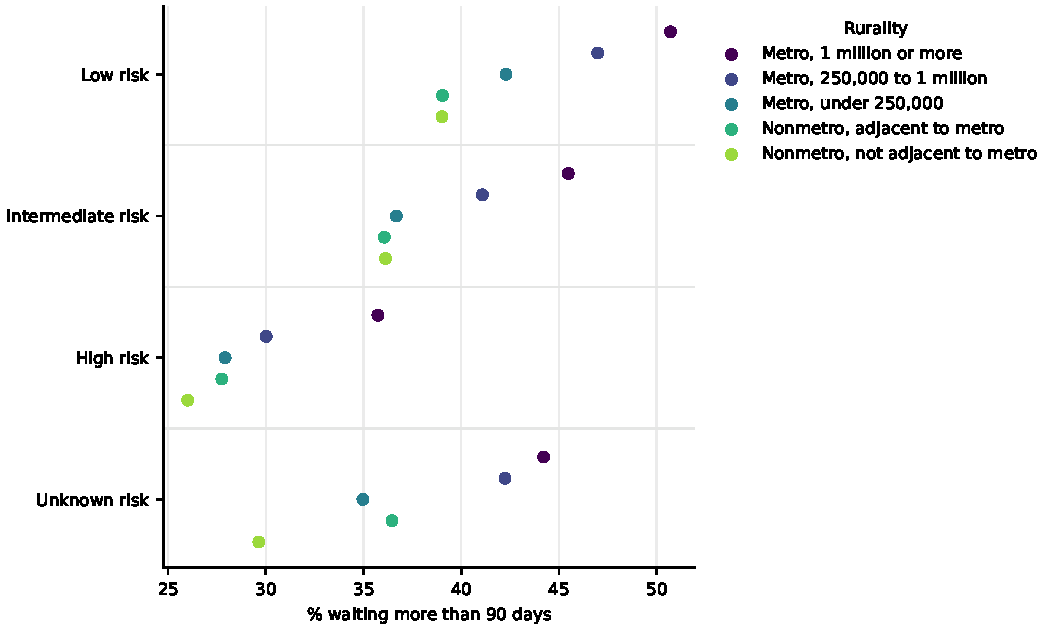
\includegraphics[width=\textwidth]{../figures/figure2_delay_by_risk_and_rurality.pdf}
\caption{Crude percentage of men waiting more than 90 days from diagnosis to first recorded treatment, by risk group and county rurality. Men with unknown rurality, and percentages resting on 1 to 4 men, are not shown. Nothing is adjusted.}
\label{fig:s1}
\end{figure}

\begin{figure}[H]
\centering
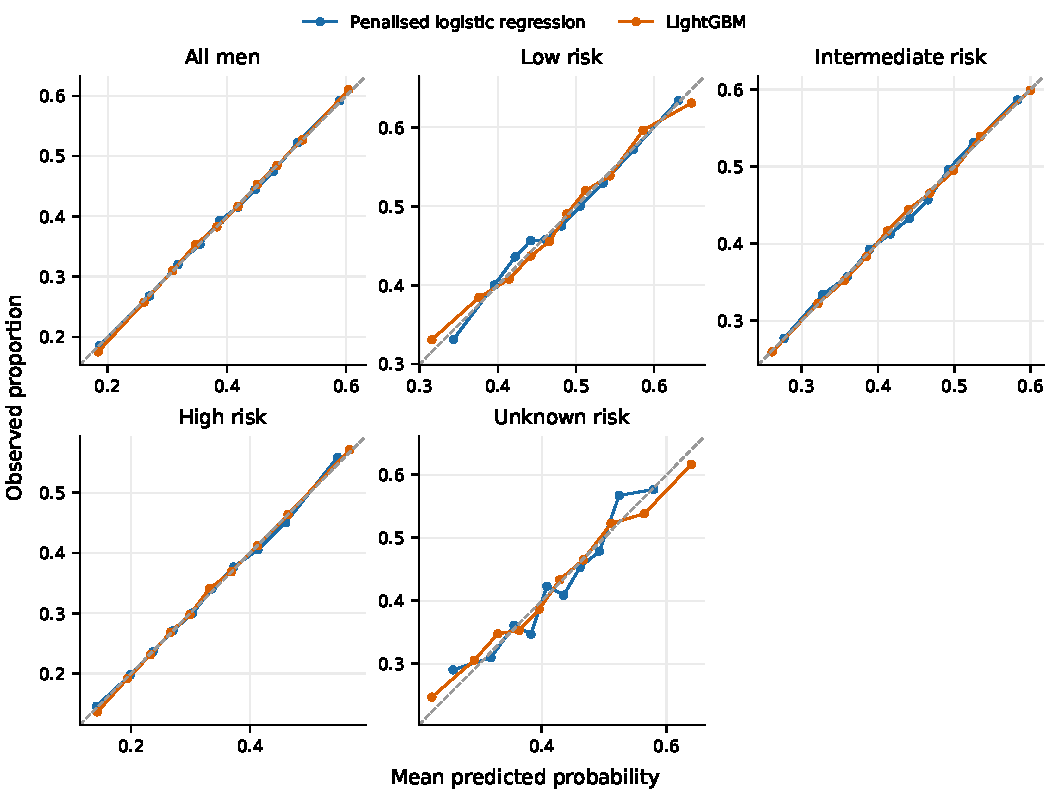
\includegraphics[width=\textwidth]{../figures/figureS1_calibration.pdf}
\caption{Calibration of out-of-fold predicted probabilities at step 2 (clinical need plus area and marital characteristics), in 10 equal-count bins, by risk group and model type. The dashed line marks perfect calibration.}
\label{fig:s2}
\end{figure}

\begin{figure}[H]
\centering
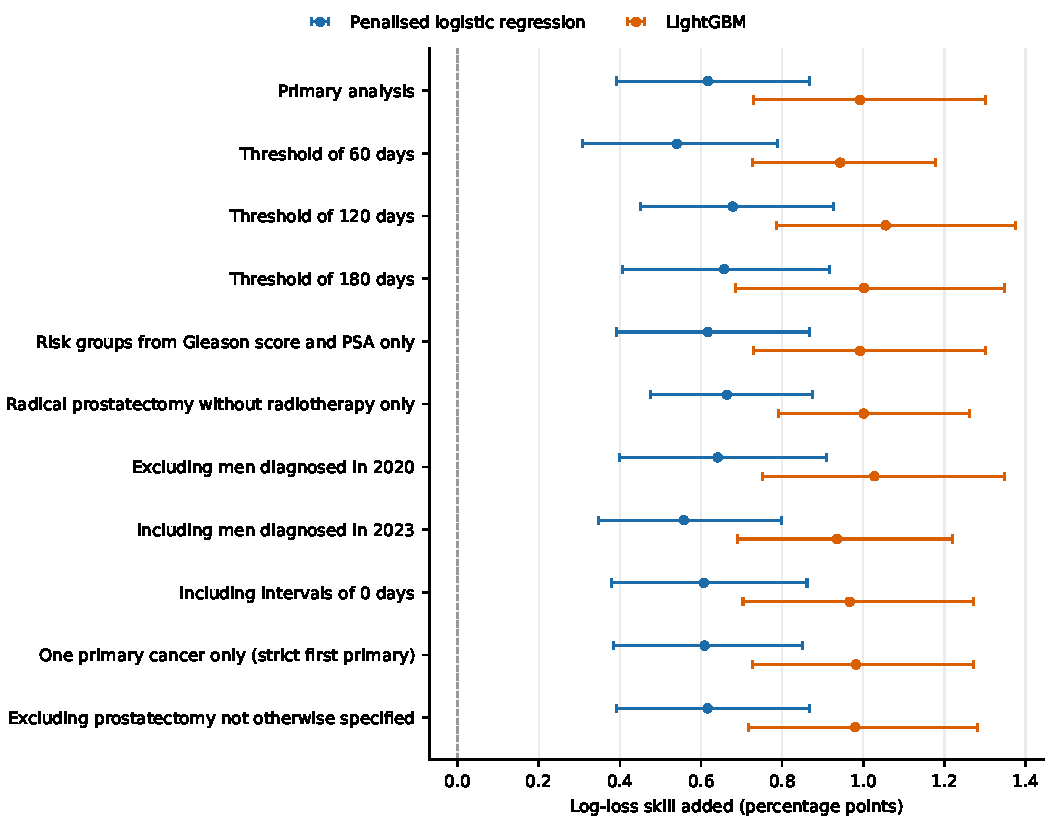
\includegraphics[width=\textwidth]{../figures/figureS2_sensitivity.pdf}
\caption{Log-loss skill added by the area and marital block under each sensitivity scenario, all men, with 95\% cluster bootstrap intervals. Each scenario changes one setting from the primary analysis. The threshold scenarios use a different outcome, so their values are not directly comparable with the others.}
\label{fig:s3}
\end{figure}

\clearpage
\section{Reporting checklists}

{\footnotesize
\begin{longtable}{@{}>{\raggedright}p{2.3cm}>{\raggedright}p{5.0cm}>{\raggedright\arraybackslash}p{7.8cm}@{}}
\caption{STROBE and RECORD checklist. Item wording is abbreviated from the RECORD statement, which includes the STROBE items~\cite{strobe2007,record2015}. Locations are sections of the main text unless marked S (this supplement).}\label{tab:strobe}\\
\toprule
\rowcolor{tablehead}Item & Topic & Where reported \\
\midrule
\endfirsthead
\toprule
\rowcolor{tablehead}Item & Topic & Where reported \\
\midrule
\endhead
1a, 1b & Design in title or abstract; informative abstract & Abstract (retrospective cohort study) \\
RECORD 1.1 to 1.3 & Database, region and time frame; linkage & Title; Abstract; Methods, Data and cohort (county attributes linked by SEER; no person-level linkage) \\
2, 3 & Background; objectives & Introduction \\
4, 5 & Study design; setting and dates & Methods, Data and cohort \\
6a & Eligibility and selection & Methods, Data and cohort; Figure 1 \\
6b & Matching & Not applicable \\
RECORD 6.1 to 6.3 & Selection codes; their validation; linkage flow & Methods, Data and cohort (codes in \texttt{config/analysis.yaml}); no validation study of the cohort algorithm; no person-level linkage \\
7, RECORD 7.1 & Outcomes and predictors; complete list of codes & Methods, Outcome and risk groups, and Ordered feature steps; \texttt{config/analysis.yaml} \\
8 & Data sources and measurement & Methods, Data and cohort, and Outcome and risk groups \\
9 & Efforts to address bias & Methods, Robustness, selection and secondary outcome; Discussion (limitations) \\
10 & Study size & Methods, Data and cohort (all eligible men); Figure 1 \\
11 & Quantitative variables & Methods, Ordered feature steps \\
12a, 12b & Statistical methods; subgroups and interactions & Methods, Models and validation (risk-group strata; clinical interaction terms), and Standardised percentages and income concentration \\
12c & Missing data & Methods, Ordered feature steps, Models and validation, and Robustness, selection and secondary outcome (bounds and weighting); Table S8 \\
12d & Loss to follow-up & Not applicable (top-coded intervals counted as delayed) \\
12e & Sensitivity analyses & Methods, Robustness, selection and secondary outcome; Tables S3 to S5 \\
RECORD 12.1 to 12.3 & Database access; data cleaning; linkage & Full case listing of the selected site and years; every export label mapped explicitly in code; no person-level linkage \\
13a to 13c, RECORD 13.1 & Numbers at each stage; flow diagram & Results, Cohort and delay; Figure 1 \\
14a, 14b & Characteristics; missing data & Table 1 (unknown categories shown) \\
14c & Follow-up time & Not applicable \\
15 & Outcome data & Results, Cohort and delay; Table S1 \\
16a & Estimates and precision & Table 2 (intervals); standardised contrasts without intervals, stated in Results; Table S6 \\
16b, 16c & Category boundaries; absolute measures & Methods, Outcome and risk groups; Table 1; Results, Standardised differences and income concentration \\
17 & Other analyses & Results, Robustness, selection and secondary outcome; Tables S3 to S9 \\
18, 20 & Key results; interpretation & Discussion \\
19, RECORD 19.1 & Limitations, including routinely collected data & Discussion, limitations paragraph \\
21 & Generalisability & Discussion \\
22 & Funding & Declarations \\
RECORD 22.1 & Access to protocol, data and code & Methods, Protocol, reporting and disclosure; Declarations \\
\bottomrule
\end{longtable}
}

{\footnotesize
\begin{longtable}{@{}>{\raggedright}p{2.3cm}>{\raggedright}p{5.0cm}>{\raggedright\arraybackslash}p{7.8cm}@{}}
\caption{TRIPOD+AI checklist. Item wording is abbreviated from the TRIPOD+AI checklist~\cite{tripodai2024}. Development and internal evaluation use the same data through cross-fitting; the models are measurement tools and are not proposed for clinical use.}\label{tab:tripod}\\
\toprule
\rowcolor{tablehead}Item & Topic & Where reported \\
\midrule
\endfirsthead
\toprule
\rowcolor{tablehead}Item & Topic & Where reported \\
\midrule
\endhead
1, 2 & Title; abstract & Title; Abstract \\
3a to 3c, 4 & Context; intended purpose; known inequalities; objectives & Introduction; Methods, Protocol, reporting and disclosure (not for clinical use) \\
5a, 5b, 6a to 6c & Data sources, dates, setting, eligibility, treatments & Methods, Data and cohort, and Ordered feature steps (treatment type at step 3) \\
7 & Data preparation & Code in the repository \\
8a to 8c & Outcome; assessors; blinding & Methods, Outcome and risk groups; assessors and blinding not applicable (registry-abstracted outcome) \\
9a to 9c & Predictors & Methods, Ordered feature steps (pre-specified in the protocol); assessors not applicable \\
10, 11 & Sample size; missing data & Methods, Data and cohort (all eligible men), Ordered feature steps, and Models and validation \\
12a to 12c & Data use; predictor handling; model type, tuning and internal validation & Methods, Models and validation (5-fold cross-fitting) \\
12d, 23b & Heterogeneity across clusters & Cluster bootstrap only; heterogeneity across clusters not examined \\
12e & Performance measures & Methods, Models and validation; Table S2; Figure S2 \\
12f, 24 & Model updating & Not applicable \\
12g & How predictions were calculated & Code in the repository \\
13 & Class imbalance & No class imbalance methods used \\
14 & Fairness & Not addressed as a model property; area and marital differences are the measured quantity \\
15 & Model output & Predicted probabilities; no classification threshold \\
16 & Training versus evaluation differences & Not applicable (cross-fitting within the same data) \\
17, 18a to 18f, 19 & Ethics; funding; conflicts; protocol; registration; data and code; patient involvement & Methods, Protocol, reporting and disclosure (not registered); Declarations \\
20a, 20b & Participant flow; characteristics & Results, Cohort and delay; Figure 1; Table 1 \\
20c & Comparison with development data & Not applicable \\
21 & Participants and events per analysis & Table 1; Table 2; Table S1 \\
22 & Full model specification & Not released as a clinical model; code that refits every model is in the repository \\
23a & Performance with intervals, including subgroups & Table 2 and Table S2 by risk group (AUC and calibration without intervals); not reported by area or marital subgroup \\
25, 26 & Interpretation; limitations & Discussion \\
27a to 27c & Implementation; next steps & Not applicable (no implementation proposed); Discussion \\
\bottomrule
\end{longtable}
}

{\small
\begin{thebibliography}{9}
\setlength{\itemsep}{0.1em}
\bibitem{zheng2023} Zheng Q, Otahal P, Cox IA, et al. The influence of immortal time bias in observational studies examining associations of antifibrotic therapy with survival in idiopathic pulmonary fibrosis: a simulation study. Front Med (Lausanne). 2023;10:1157706.
\bibitem{foley2022} Foley GR, Blizzard CL, Stokes B, et al. Urban-rural prostate cancer disparities in a regional state of Australia. Sci Rep. 2022;12(1):3022.
\bibitem{foley2025} Foley GR, Blizzard CL, Skala M, et al. Prostate cancer disparities between public and private healthcare patients in Tasmania, a regional state of Australia. Cancers (Basel). 2025;18(1):79.
\bibitem{strobe2007} von Elm E, Altman DG, Egger M, et al. The Strengthening the Reporting of Observational Studies in Epidemiology (STROBE) statement: guidelines for reporting observational studies. Lancet. 2007;370:1453-7.
\bibitem{record2015} Benchimol EI, Smeeth L, Guttmann A, et al. The REporting of studies Conducted using Observational Routinely-collected health Data (RECORD) statement. PLoS Med. 2015;12(10):e1001885.
\bibitem{tripodai2024} Collins GS, Moons KGM, Dhiman P, et al. TRIPOD+AI statement: updated guidance for reporting clinical prediction models that use regression or machine learning methods. BMJ. 2024;385:e078378.
\end{thebibliography}
}

\end{document}
